\documentclass{article}
\usepackage[utf8]{inputenc}
\usepackage{amssymb, mathtools, amsmath}
\usepackage[dvipsnames]{xcolor}
\usepackage{graphicx}
\usepackage{float}
\usepackage{caption}
\usepackage{hyperref}
\hypersetup{
    colorlinks=true,
    linkcolor=blue,
    filecolor=magenta,      
    urlcolor=blue,
}

\title{ Macroeconomic Theory
        \thanks{Course instructed by Professor Christoph Hedtrich.} \\
        Homework 4: Consumption Decisions
        }

\author{
        % Add your name here
        Uppsala Masters in Economics 2021-2022
        }

\date{25 November 2021}

% margins
\oddsidemargin 3mm
\evensidemargin 3mm
\topmargin -12mm
\textheight 600pt
\textwidth 420pt

% no indent
\setlength\parindent{0pt}
% \renewcommand{\theenumi}{\thesection(\alph{enumi})}
% \renewcommand\thesubsection{\arabic{subsection}}

% custom commands
\newcommand{\E}[1]{\mathrm{E}\left[#1\right]}
\newcommand{\cov}[1]{\mathrm{Cov}\left(#1\right)}
\newcommand{\var}[1]{\mathrm{Var}\left(#1\right)}
\renewcommand{\L}{\mathcal{L}}

\begin{document}
    
    \maketitle
    
    \section{Consumption: Permanent Income Hypothesis}
    
    \subsection{Consumer utility}
    
        Individual lives for $T$ periods, lifetime utility is given by
        \begin{align}
            U = \sum_{t=1}^T u(C_t), \quad u'(\cdot) > 0, \quad u'(\cdot) < 0,
        \end{align}
        
        subject to the constraint
        \begin{align}
            \sum_{t=1}^T C_t \le A_0 + \sum_{t=1}^T Y_t, \label{eqn:constant-budget}
        \end{align}
        where $A_0$ is initial wealth, and $C_t, Y_t$ are consumption and income at time $t$. Form the Lagrangian
        \begin{align}
            \L\left(\{C_t\}_{t=1}^{T}, \lambda\right)
            &=\sum_{t=1}^T u(C_t) + \lambda  \left(A_0 +\sum_{t=1}^T Y_t - \sum_{t=1}^T C_t \right),
        \end{align}
        
        where FOC with respect to consumption $C_t$ in any period $t = 1, ..., T$ is
        \begin{align}
            \frac{\partial \L}{\partial C_t}
            = u'(C_t^*) - \lambda
            &= 0
            \\
            \implies u'(C_t^*) &= \lambda.
        \end{align}
        
        Since $\lambda$ is constant, optimal consumption is also constant across time $t = 1, ..., T$. Then we have
        \begin{align}
            C_t^* &= {u'}^{-1}(\lambda) = \bar{C}.
        \end{align}
        
        From the budget constraint \eqref{eqn:constant-budget} (and assuming no free disposal), we have for $t = 1, ..., T$ that
        \begin{align}
            \sum_{t=1}^T C_t^*
            = \sum_{t=1}^T \bar{C}
            = T \bar{C}
            &= A_0 + \sum_{t=1}^T Y_t
            \\
            \implies
            C_t^*
            =\bar{C}
            &= \frac{1}{T} \left( A_0 + \sum_{s=1}^T Y_s \right)
            = \frac{1}{T}\sum_{s=1}^T Y_s +  \frac{A_0}{T}
        \end{align}
        
        This implies optimal consumption is not determined by income in any period $t$ but only by the total (or average) income across time. This is the \textbf{permanent-income hypothesis.}
    
    \subsection{Income and consumption fluctuations}
        
        Income $Y_{it}$ for individual $i$ at time $t$ can be represented as
        \begin{align}
            Y_{it} = Y_{i}^P + Y_{it}^T
            \label{eqn:income-fluctuation}
        \end{align}
        where $Y_{i}^P$ is the average across time or \textbf{permanent income}, and $Y_{it}^T = Y_{it} - Y_{i}^P$ is the \textbf{transitory income}, where we assume
        \begin{align}
            \sum_{t=1}^T Y_{it}^T = 0,\quad
            \cov{Y_{it}^T, Y_{i}^P} = 0.
        \end{align}
        
        Now we assume some exogenous, unexpected fluctuations in consumption. Then individual $i$ maximizes lifetime utility
        \begin{align}
            U_i &= \sum_{t=1}^T u\left(C_{it} - e_{it}\right)
             \quad s.t. \quad
            \sum_{t=1}^T \left(C_{it} - e_{it}\right) \le A_0 + \sum_{t=1}^T Y_t,
            \label{eqn:utility-fluctuation}
        \end{align}
        
        where $e_{it}$ is the \textbf{transitory consumption} (sort of like a ``consumption shock") with $\sum_{t=1}^T e_{it} = 0$. Then forming the Lagrangian, we have that
        \begin{align}
            \L
            &=
            \sum_{t=1}^T u\left(C_{it} - e_{it}\right)
            + \lambda \left[A_0 + \sum_{t=1}^T Y_t - \sum_{t=1}^T \left(C_{it} - e_{it}\right)\right]
            \\
            \frac{\partial \L}{\partial C_{it}}
            &= u'\left(C_{it}^* - e_{it}\right) - \lambda = 0
            \implies u'\left(C_{it}^* - e_{it}\right) = \lambda,
        \end{align}
        
        which implies $C_{it}^* - e_{it} = \bar{C_e}$ is constant across time also. Then with the budget constraint in \eqref{eqn:utility-fluctuation}, we have that
        
        \begin{align}
            \sum_{t=1}^T \left(C_{it} - e_{it}\right)
            &= A_0 + \sum_{t=1}^T Y_{it}
            \\ \implies
            \sum_{t=1}^T C_e
            &= A_0 + \sum_{t=1}^T (Y_{i}^P + Y_{it}^T)
            \\
            &= A_0 + \sum_{t=1}^T Y_{i}^P + \sum_{t=1}^T Y_{it}^T
            \\ \implies
            \sum_{t=1}^T \bar{C_e}
            = T \bar{C_e}
            &= A_0 + T \cdot Y_{i}^P.
        \end{align}
        
        Assuming $A_0 = 0$, we have that
        \begin{align}
            T \bar{C_e} &= T \cdot Y_{i}^P
            \\
            \implies 
            \bar{C_e} &= Y_{i}^P
            \\
            \implies
            C_{it} - e_{it} &= Y_{i}^P, \quad t = 1, ..., T
        \end{align}    
        
        Rearranging, we have the consumption function
        \begin{align}
            C_{it} &= Y_{i}^P + e_{it}, \quad t = 1, ..., T.
            \label{consumption-fluctuation}
        \end{align}
    
        Running an OLS linear regression on $C_{it}$ with $Y_{it}$, we have
        \begin{align}
            C_{it} &= a + b Y_{it} + u_{it}
            \label{eqn:consumption-regression}
        \end{align}
        
        where with permanent income \eqref{eqn:income-fluctuation} and consumption \eqref{consumption-fluctuation}, we have
        \begin{align}
            \cov{x, y} &= \frac{1}{N}\sum_{i=1}^N(x_i - \bar{x})(y_i - \bar{y}) \\
            \var{y} &= \frac{1}{N}\sum_{i=1}^N(y_i - \bar{y})^2
        \end{align}
        \begin{align}
            \hat{b}
            = \frac{ \cov{Y_{it}, C_{it}} }{ \var{Y_{it}} }
            &= \frac{ \cov{Y_{i}^P + Y_{it}^T, Y_{i}^P + e_{it}} }{ \var{Y_{i}^P + Y_{it}^T} }
            % &= \frac{ \cov{Y_{i}^P, Y_{i}^P} }{ \var{Y_{i}^P} + \var{Y_{it}^T} }
            \\
            &= \frac{ \var{Y_{i}^P} }{ \var{Y_{i}^P} + \var{Y_{it}^T} }
            \label{eqn:regression-bhat}
        \end{align}
        
        and 
        \begin{align}
            \hat{a}
            = \E{C_{it}} - \hat{b}\E{Y_{it}}
            &= \E{Y_{i}^P + e_{it}} - \hat{b}\E{Y_{i}^P + Y_{it}^T}
            \\
            &= \E{Y_{i}^P} + \E{e_{it}} - \hat{b}\left(\E{Y_{i}^P} + \E{Y_{it}^T}\right)
            \\
            &= \left(1 - \hat{b}\right) \E{Y_{i}^P}.
            \label{eqn:regression-ahat}
        \end{align}

    % \subsection{Savings}
    % Individual savings is
    % \begin{align}
    %     S_t &= Y_t - C_t
    %     \\
    %     &= Y_t -  \frac{1}{T} \left( A_0 + \sum_{s=1}^T Y_s \right)
    %     \\
    %     &= \left(Y_t -  \frac{1}{T}\sum_{s=1}^T Y_s \right) +  \frac{A_0}{T}
    %     \\
    %     &= \left(Y_t -  \bar{Y} \right) +  \frac{A_0}{T}
    % \end{align}
    
    % where $\bar{Y}$ is the average income in all periods.
        
    
    \subsection{Question 1: DR 8.2.}
        
        \begin{figure}[!h]
            \centering
            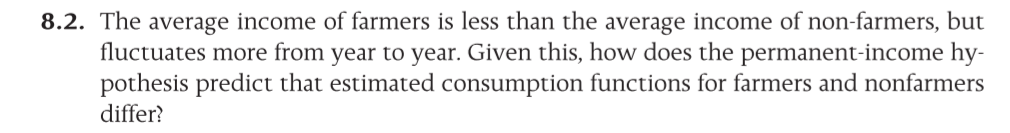
\includegraphics[width=\textwidth]{./HW4-DR8.2.png}
        \end{figure}
        
        For income of farmers $Y_F$ and non-farmers $Y_{NF}$, we have
        \begin{align}
            \E{Y_F} &< \E{Y_{NF}}, \quad
            \var{Y_F} > \var{Y_{NF}}.
            \label{eqn:farmers-nonfarmers}
        \end{align}
        
        Assume consumption functions of farmers $C_{F}$ and non-farmers $C_{NF}$ are linear in their income like \eqref{eqn:consumption-regression}, with the form
        \begin{align}
            C_{F} &= a_{F} + b_{F} Y_{F} + u_{F},
            \\
            C_{NF} &= a_{NF} + b_{NF} Y_{NF} + u_{NF}.
        \end{align}
        
        Then by \eqref{eqn:regression-bhat} and \eqref{eqn:regression-ahat} the parameters are
        \begin{align}
            \hat{b}_{F} &= \frac{\var{Y_{F}^P}}{\var{Y_{F}^P} + \var{Y_{F}^T}},
            \quad
            \hat{a}_{F} = \left(1 - \hat{b}_{F}\right) \E{Y_{F}^P},
            \\
            \hat{b}_{NF} &= \frac{\var{Y_{NF}^P}}{\var{Y_{NF}^P} + \var{Y_{NF}^T}},
            \quad
            \hat{a}_{NF} = \left(1 - \hat{b}_{NF}\right) \E{Y_{NF}^P}.
        \end{align}
        
        Since $\var{Y_{it}} = \var{Y_{i}^P} + \var{Y_{it}^T}$ and \eqref{eqn:farmers-nonfarmers}, we have that if
        
        \begin{itemize}
            \item 
            $\var{Y_{F}^P} = \var{Y_{NF}^P} \implies \var{Y_{F}^T} > \var{Y_{NF}^T} \implies \hat{b}_{F} < \hat{b}_{NF}$, relative size of $\hat{a}$ is ambiguous.
            
            \item
            $\var{Y_{F}^P} < \var{Y_{NF}^P} \implies \var{Y_{F}^T} > \var{Y_{NF}^T} \implies \hat{b}_{F} < \hat{b}_{NF}$, relative size of $\hat{a}$ is ambiguous.
            
            \item
            If $\var{Y_{F}^P} > \var{Y_{NF}^P}$, then relative sizes of $\hat{b}$ and $\hat{a}$ are ambiguous.
        \end{itemize}
        
        % By \eqref{consumption-fluctuation}, the consumption functions of farmers $f$ and non-farmers $n$ for periods $t = 1, ..., T$ are
        % \begin{align}
        %     C_{ft} &= Y_{f}^P + e_{ft},
        %     \\
        %     C_{nt} &= Y_{n}^P + e_{nt},
        % \end{align}
        
        % where $Y_{f}^P < Y_{n}^P$, $\var(e_{ft}) > \var(e_{ft})$, and $\mathrm{E}[e_{ft}] = \mathrm{E}[e_{nt}] = 0$. This implies that
        % \begin{align}
        %     \mathrm{E}[C_{it}]
        %     &= E\left[Y_{i}^P + e_{it}\right]
        %     \\
        %     &= E\left[Y_{i}^P\right] + \mathrm{E}[e_{it}]
        %     \\
        %     &= Y_{i}^P + \mathrm{E}[e_{it}]
        %     \\
        %     &= Y_{i}^P + 0
        %     = Y_{i}^P
        % \end{align}
        % which implies average consumption $\mathrm{E}[C_{ft}] = Y_{f}^P < Y_{n}^P = \mathrm{E}[C_{nt}]$. Then the variance of consumption is
        % \begin{align}
        %     \var(C_{it})
        %     &= E\left[\left(Y_{i}^P + e_{it} - \mathrm{E}[C_{it}]\right)^2\right]
        %     \\
        %     &= E\left[\left(Y_{i}^P + e_{it} - Y_{i}^P\right)^2\right]
        %     = E\left[e_{it}^2\right]
        %     \\
        %     &= \var(e_{it}),
        % \end{align}
        
        % which implies $\var(C_{ft}) = \var(e_{ft}) > \var(e_{ft}) = \var(C_{nt})$.
        
    
    \newpage
    \section{Government Spending and Uncertainty}
    
    \subsection{Question 2: DR 8.7.}
        
        \begin{figure}[!h]
            \centering
            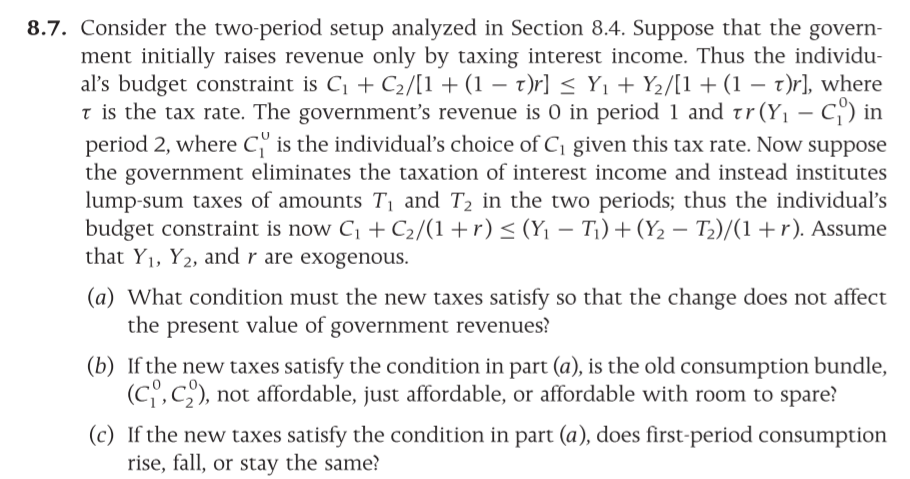
\includegraphics[width=\textwidth]{./HW4-DR8.7.png}
        \end{figure}
        
        \begin{itemize}
            \item[(a)]
            For present value of government revenues to be the same between the interest and lump-sum tax, then
            \begin{align}
                G^0 = \frac{1}{1+r} \tau (Y_1 - C_1^0)
                &= T_1 + \frac{1}{1+r} T_2.
            \end{align}
            
            
            \item[(b)]
            The old bundle \boxed{(C_1^0, C_2^0) \text{ is just affordable,}} since the total after-tax budget does not change (lump-sum taxes paid are the same as interest taxes).
            
            % \begin{align}
            %     Y_1 + \frac{Y_2}{1 + (1-\tau)r}
            %     &= C_1^0 + \frac{C_2^0}{(1 - \tau)r}
            %     \\
            %     &= C_1^0 + \frac{C_1^0\left(\frac{1 + (1-\tau)r}{1-\rho}\right)^{1/\theta}}{(1 - \tau)r}
            % \end{align}
            
            
            
            \item[(c)]
            For two period model, given whichever tax policy, consumption objective is to maximize
            \begin{align}
                U &= \frac{C_1^{1-\theta}}{1-\theta} + \frac{1}{1+\rho} \frac{C_2^{1-\theta}}{1-\theta},
                \quad \theta \in [0, 1)
                \\ s.t. \quad &
                C_1 + \frac{C_2}{1 + (1-\tau)r}
                \le 
                (Y_1 - T_1) + \frac{(Y_2 - T_2)}{1 + (1-\tau)r},
                \quad \tau \in [0, 1]
            \end{align}
            
            Forming the Lagrangian,
            \begin{align}
                \L
                &= \frac{C_1^{1-\theta}}{1-\theta} + \frac{1}{1+\rho} \frac{C_2^{1-\theta}}{1-\theta}
                + \lambda \left( (Y_1 - T_1) + \frac{(Y_2 - T_2)}{1 + (1-\tau)r} - C_1 - \frac{C_2}{1 + (1-\tau)r} \right),
            \end{align}
            we have with the FOCs that
            \begin{align}
                \frac{\partial \L}{\partial C_1} = 0
                &\implies
                C_1^{-\theta} = \lambda \\
                \frac{\partial \L}{\partial C_2} = 0
                &\implies
                \frac{1}{1+\rho}C_2^{-\theta} = \frac{\lambda}{1 + (1-\tau)r}
                \\ &\implies
                \frac{1 + (1-\tau)r}{1+\rho}C_2^{-\theta} = \lambda  = C_1^{-\theta}
                \\ &\implies
                \frac{C_2}{C_1} = \left(\frac{1 + (1-\tau)r}{1+\rho}\right)^{1/\theta},
            \end{align}
            
            which is the Euler equation. We can then see that
            \begin{align}
                \frac{\partial (C_2 / C_1)}{\partial \tau}
                = -\frac{r}{1+\rho}\frac{1}{\theta}\left(\frac{1 + (1-\tau)r}{1+\rho}\right)^{\frac{1}{\theta} - 1}
                < 0.
            \end{align}
            Thus a reduction in interest tax rate $\tau$ to zero will result in an increase in $C_2/C_1$, and the first period consumption \boxed{C_1 \text{ will fall}} (relative to the second period).
            
            
            
            
        \end{itemize}
        
\end{document}
